\documentclass[aspectratio=169,xcolor=table]{beamer}
\usepackage{algorithm}
\usepackage{algpseudocode}
\usepackage[utf8]{inputenc}
\usepackage[T1]{fontenc}
\usepackage{lmodern}
\usepackage{csquotes}
\usepackage{xcolor}
\usepackage[portuguese]{babel}
\usepackage[backend=biber,style=numeric]{biblatex}
\addbibresource{Bibliografia.bib}
\usepackage{graphicx}

% ------------------------------------------------
% Tema do Beamer (exemplo de um tema customizado)
% ------------------------------------------------
\usetheme{DCC} % <-- Ajuste conforme seu tema ou estilo

\graphicspath{{imgs/}{../resultados/}}
\graphicspath{{imgs/}{../Figuras/}}

\author[Chaves, Leahy]{%
  \textbf{João Pedro Chaves} \\
  \textbf{João Victor Leahy}
}
\title{Renderização Híbrida: Combinando o Melhor de Dois Mundos \\ \large{MATA65 - Computação Gráfica}}
\institute{Universidade Federal da Bahia \\ Instituto de Computação}
\date{\today}

\begin{document}

%-------------------------------------------------
%  SLIDE DE TÍTULO
%-------------------------------------------------
\begin{frame}[plain,noframenumbering]
    \titlepage
\end{frame}

%-------------------------------------------------
%  SLIDE DE AGENDA
%-------------------------------------------------
\begin{frame}{Agenda}
    \tableofcontents[hideallsubsections]
\end{frame}

%=================================================
\section{Introdução}
%=================================================
\begin{frame}{Introdução}
    \begin{itemize}
        \item A demanda por gráficos realistas em jogos e simulações cresce continuamente.
        \item A renderização híbrida combina rasterização e ray tracing para obter o melhor de cada técnica.
        \item A modularização permite otimizar cada aspecto visual individualmente, resultando em maior eficiência e qualidade.
    \end{itemize}
\end{frame}

\begin{frame}{Exemplo de Renderização Híbrida}
    \begin{center}
        \includegraphics[height=0.8\textheight]{exemplo-cena-realista}
    \end{center}
    \begin{center}
        \small{Cena renderizada utilizando técnicas híbridas, demonstrando reflexos, sombras suaves e iluminação global}
    \end{center}
\end{frame}

%=================================================
\section{Conceitos Fundamentais}
%=================================================
\begin{frame}{Arquitetura Modular: O Pipeline Híbrido}
    \begin{itemize}
        \item O pipeline é dividido em etapas que se conectam, onde a saída de uma etapa serve como entrada para a próxima.
        \item A interoperabilidade do DirectX permite o compartilhamento de dados intermediários entre as etapas.
        \item A abordagem é escalável, adaptando as técnicas à capacidade do hardware.
        \item Cada etapa utiliza a técnica mais apropriada: rasterização, ray tracing ou computação.
    \end{itemize}
\end{frame}

\begin{frame}{Pipeline de Renderização Híbrida}
    \begin{center}
        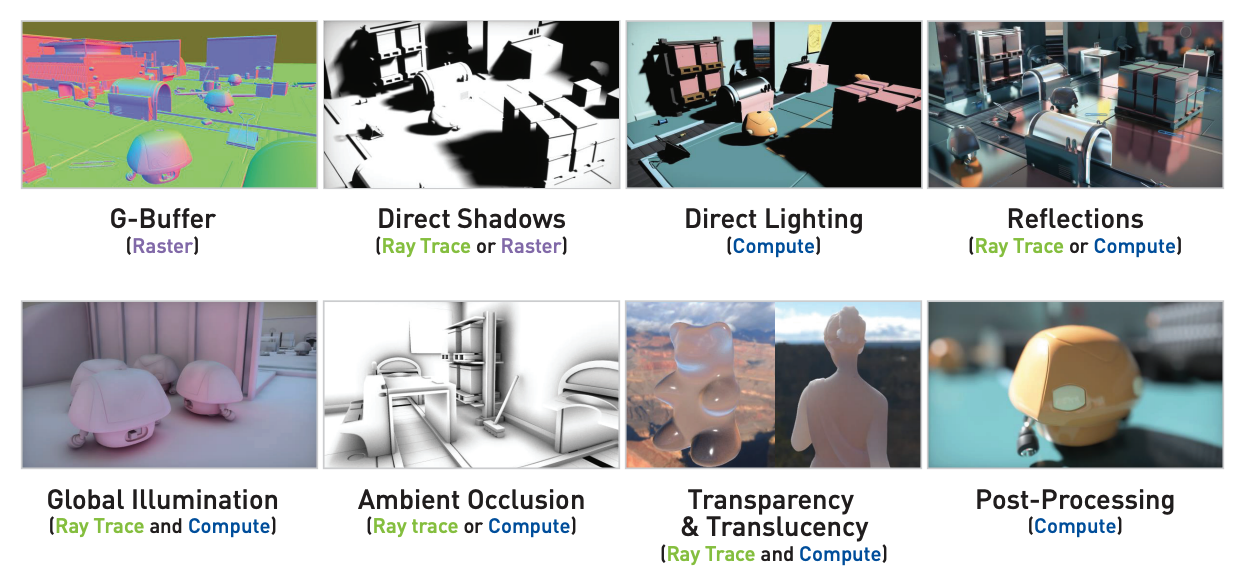
\includegraphics[height=0.8\textheight]{pipeline}
    \end{center}
    \begin{center}
        \small{G-Buffer (Raster) → Sombras Diretas (Ray Trace/Raster) → Iluminação Direta (Compute) → \\
        Reflexos (Ray Trace/Compute) → Iluminação Global → Oclusão Ambiente → Transparência → Pós-Processamento}
    \end{center}
\end{frame}

\begin{frame}{Sombras Realistas: Ray Tracing e Filtragem}
    \begin{itemize}
        \item Raios são lançados da superfície para a luz para determinar a ocultação.
        \item O ângulo do cone cria penumbras suaves, com um custo de ruído.
        \item O ruído é removido com filtragem espacial e temporal (SVGF).
        \item Sombras transparentes acumulam absorção de luz ao longo do trajeto.
    \end{itemize}
    \begin{equation*}
        \text{SombraFiltrada}(x) = \text{SVGF}(\text{Sombra}(x), \text{Variância}(x))
    \end{equation*}
\end{frame}

\begin{frame}{Comparação de Sombras Híbridas}
    \begin{center}
        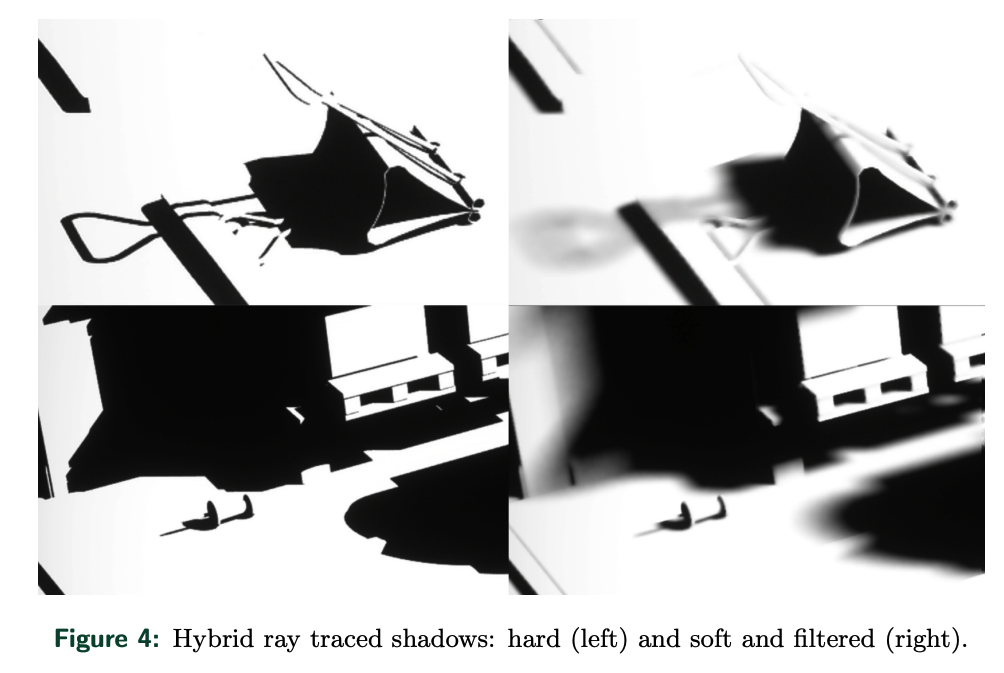
\includegraphics[height=0.8\textheight]{shadow-filter}
    \end{center}
    \begin{center}
        \small{Comparação entre sombras duras (esquerda) e sombras suaves filtradas (direita)}
    \end{center}
\end{frame}

\begin{frame}{Processo de Filtragem de Sombras}
    \begin{center}
        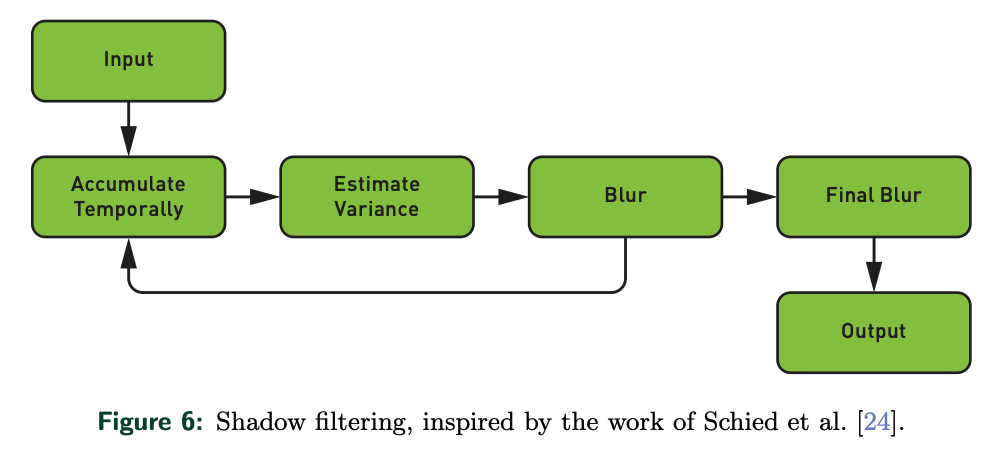
\includegraphics[width=0.9\textwidth]{shadow-filtering}
    \end{center}
    \begin{center}
        \small{Pipeline de filtragem de sombras baseado no trabalho de Schied et al. \cite{Schied2017}}
    \end{center}
\end{frame}

\begin{frame}{Acumulação de Sombras Transparentes}
    \begin{center}
        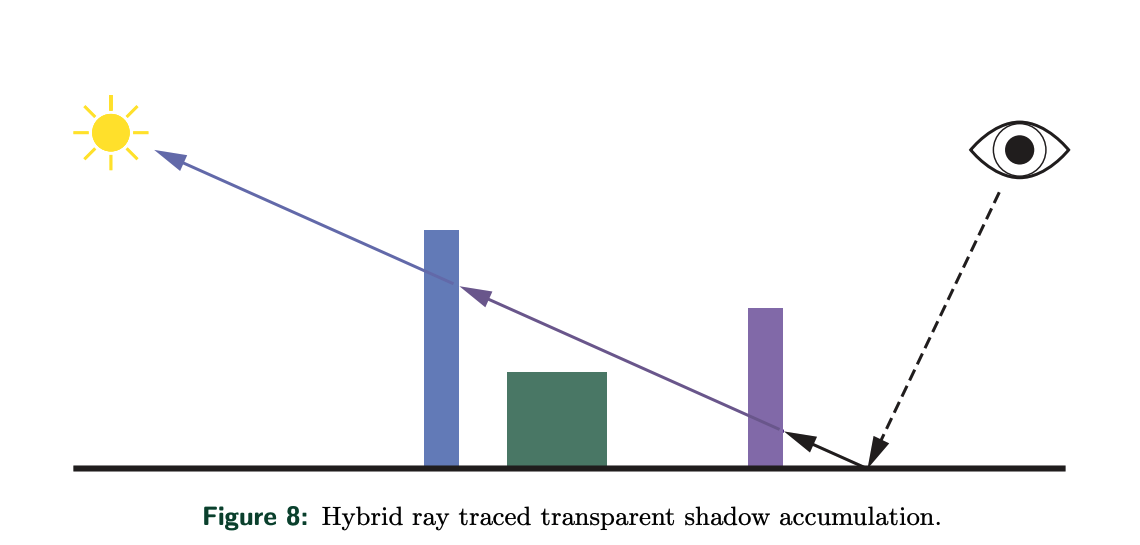
\includegraphics[height=0.7\textheight]{shadow-accumulation}
    \end{center}
    \begin{center}
        \small{Diagrama mostrando o processo de acumulação de luz em sombras transparentes}
    \end{center}
\end{frame}

\begin{frame}{Resultado: Sombras Transparentes}
    \begin{center}
        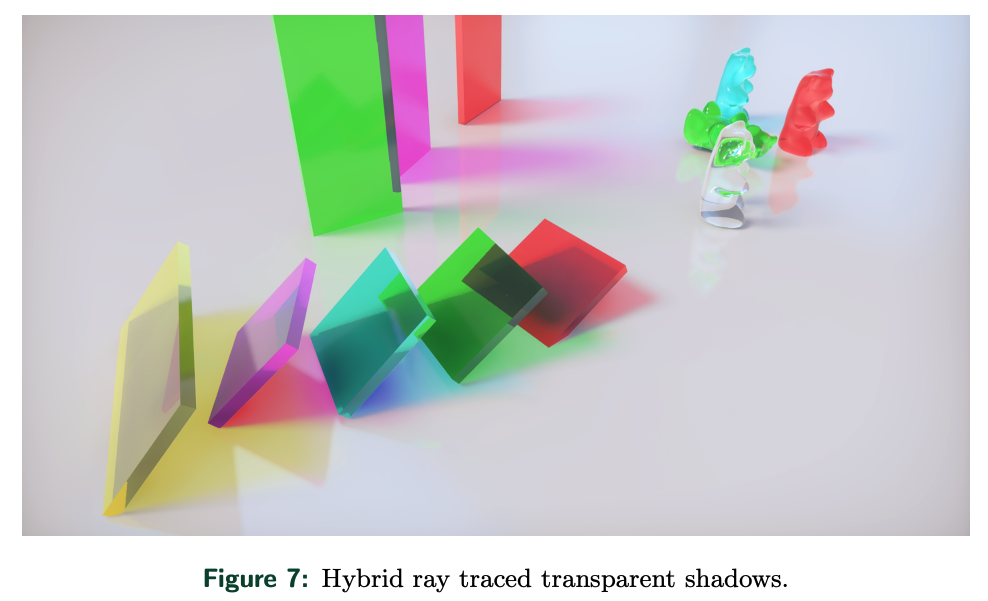
\includegraphics[height=0.8\textheight]{transparent-shadow}
    \end{center}
    \begin{center}
        \small{Exemplo de sombras transparentes coloridas com ray tracing híbrido}
    \end{center}
\end{frame}

\begin{frame}{Reflexos Dinâmicos com Ray Tracing}
    \begin{itemize}
        \item Ray tracing gera reflexos precisos sem as limitações do SSR.
        \item A amostragem de importância gera raios refletidos com base no BRDF do material.
        \item O modelo de material combina múltiplas camadas em um BRDF unificado.
    \end{itemize}
\end{frame}

\begin{frame}{Exemplo de Reflexos com Ray Tracing}
    \begin{center}
        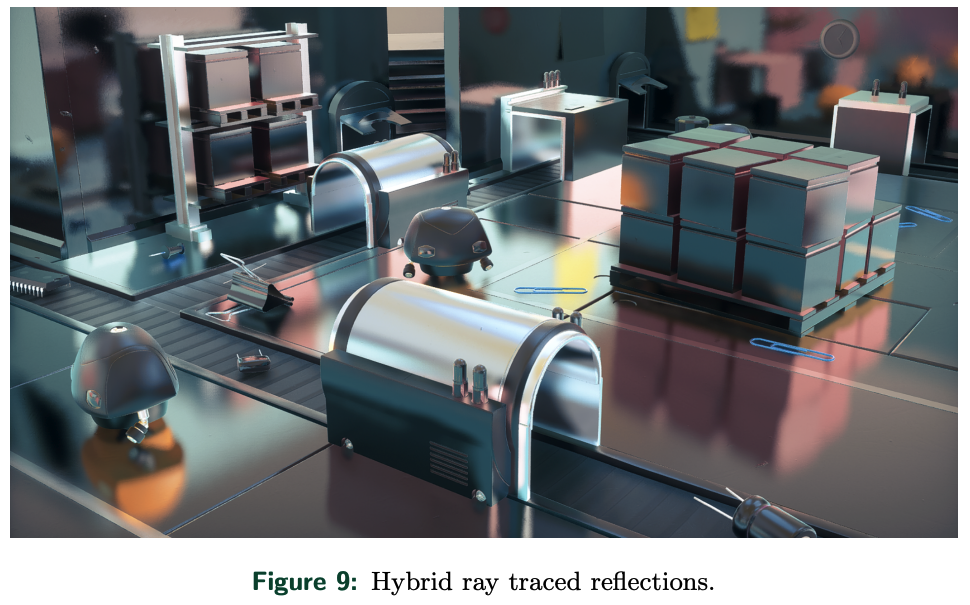
\includegraphics[height=0.8\textheight]{reflections}
    \end{center}
    \begin{center}
        \small{Reflexos precisos em superfícies metálicas usando ray tracing híbrido}
    \end{center}
\end{frame}

\begin{frame}{Pipeline de Processamento de Reflexos}
    \begin{center}
        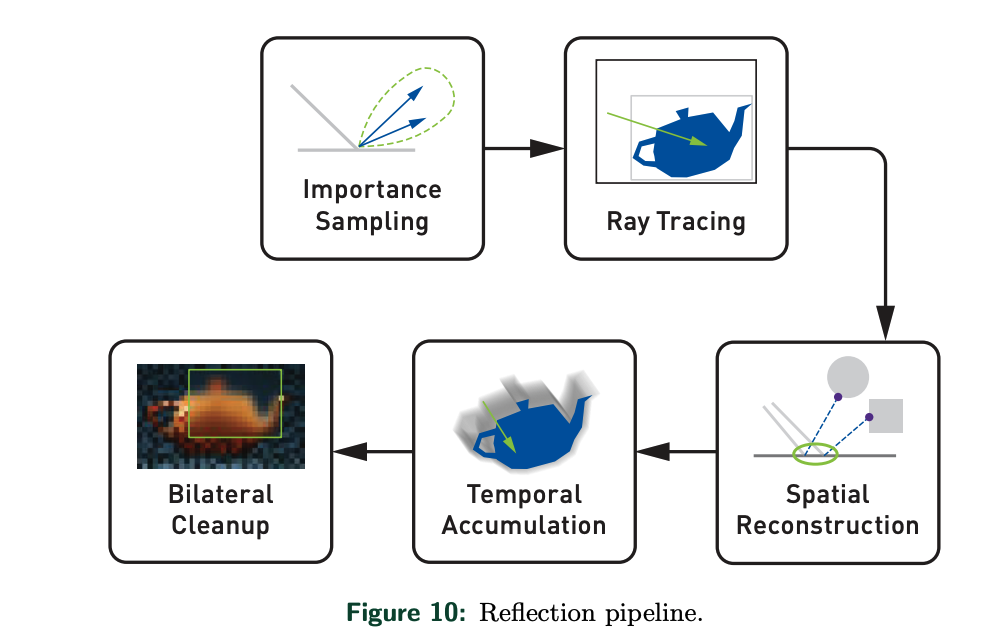
\includegraphics[width=0.95\textwidth]{reflections-pipeline}
    \end{center}
    \begin{center}
        \small{Pipeline de reflexos: Amostragem de Importância → Ray Tracing → Reconstrução Espacial → Acumulação Temporal → Limpeza Bilateral}
    \end{center}
\end{frame}

\begin{frame}{Oclusão Ambiente: Aprofundando o Realismo}
    \begin{itemize}
        \item A Oclusão Ambiente (AO) simula o sombreamento em áreas de contato.
        \item Ray tracing é mais preciso que GTAO, especialmente para objetos fora da tela.
        \item Raios são lançados em um hemisfério, e a oclusão é determinada pela quantidade de raios que atingem um objeto.
    \end{itemize}
    \begin{equation*}
        \text{AO}(x) = \frac{1}{N} \sum \text{Visibilidade}(x, \omega_i)
    \end{equation*}
\end{frame}

\begin{frame}{Comparação de Técnicas de Oclusão Ambiente}
    \begin{center}
        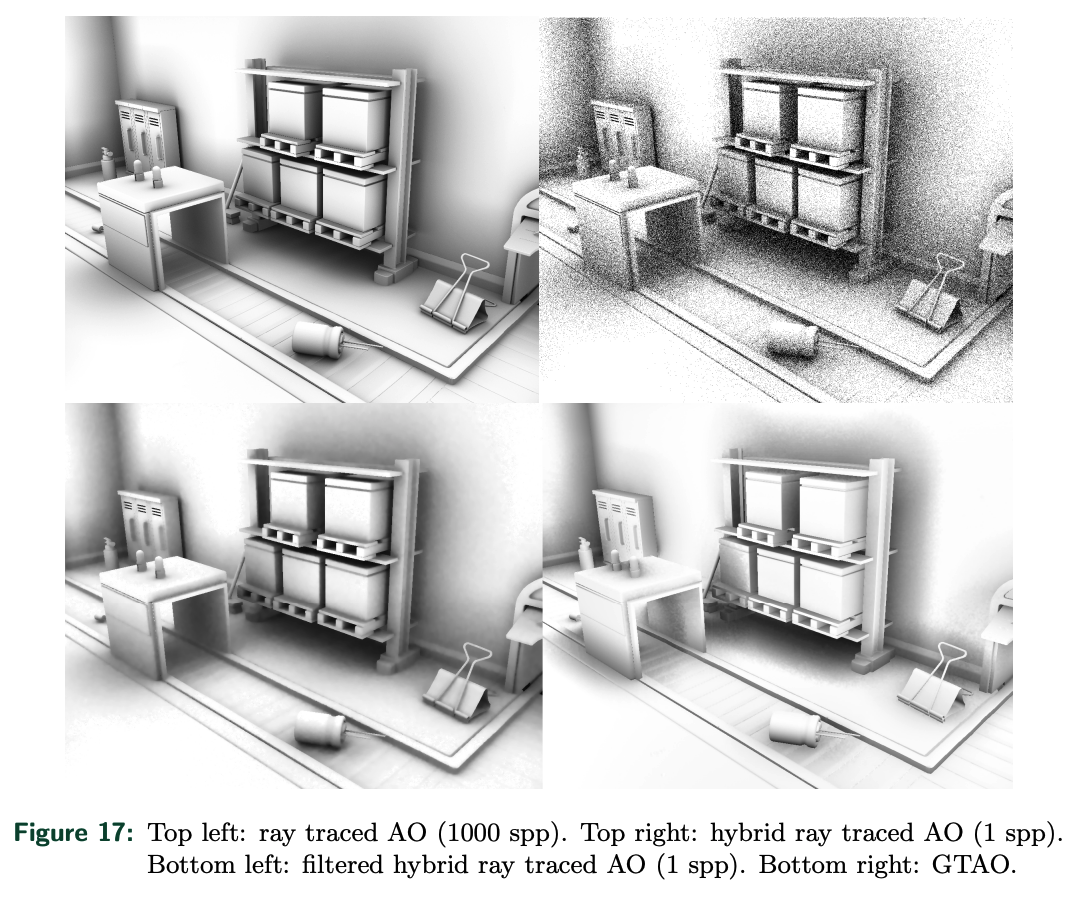
\includegraphics[height=0.7\textheight]{ambient-occlusion}
    \end{center}
    \begin{center}
        \small{Comparação de técnicas: Ray traced AO (1000 spp), Hybrid ray traced AO (1 spp),\\
        Filtered hybrid ray traced AO (1 spp), e GTAO}
    \end{center}
\end{frame}

\begin{frame}{Transparência e Translucidez: Efeitos Realistas}
    \begin{itemize}
        \item Ray tracing permite transparência sem ordem, e classifica corretamente malhas transparentes.
        \item Refração suave e áspera são tratadas com múltiplos raios para melhor convergência.
        \item Translucidez é simulada em espaço de textura, acumulando resultados ao longo do tempo.
    \end{itemize}
    \begin{equation*}
        n_1 \sin(\theta_1) = n_2 \sin(\theta_2) \text{ (Lei de Snell)}
    \end{equation*}
\end{frame}

\begin{frame}{Processo de Espalhamento de Luz}
    \begin{center}
        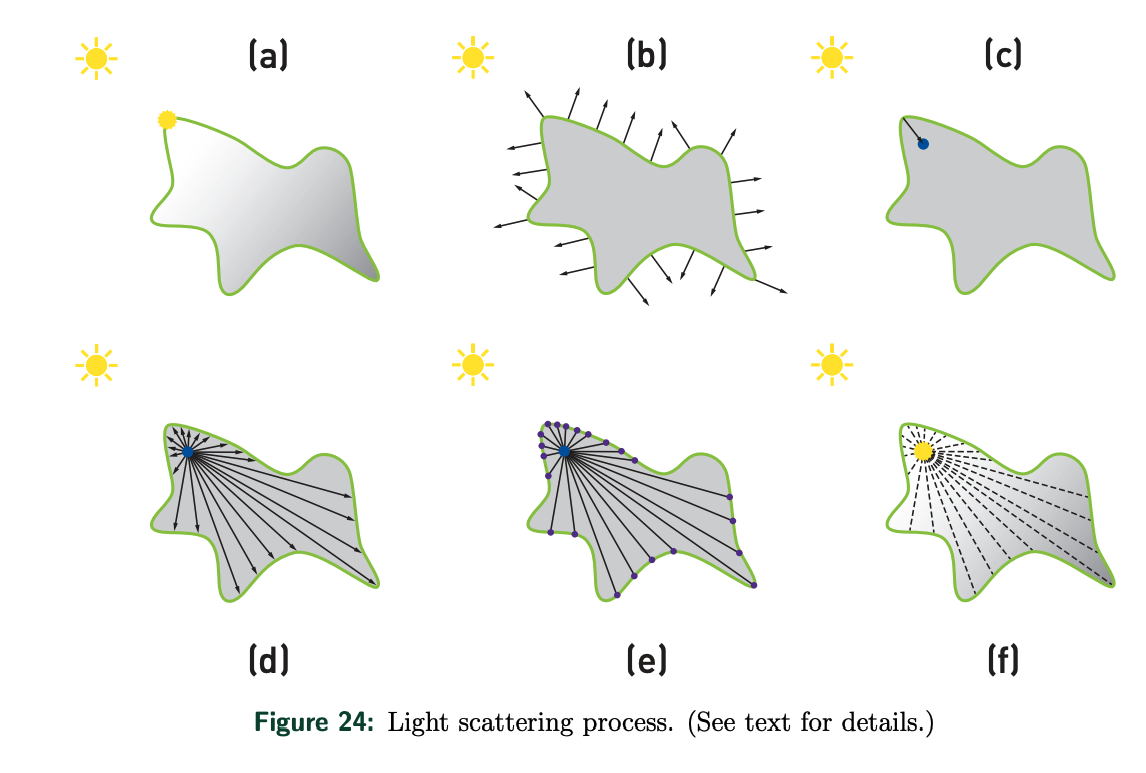
\includegraphics[width=0.95\textwidth]{light-scattering-process}
    \end{center}
    \begin{center}
        \small{Processo de espalhamento de luz em materiais: (a) reflexão direta, (b) espalhamento na superfície,\\
        (c) ponto de entrada, (d) raios de amostragem, (e) pontos de interseção, (f) raios de saída}
    \end{center}
\end{frame}

\begin{frame}{Transparência em Espaço de Objeto vs Textura}
    \begin{center}
        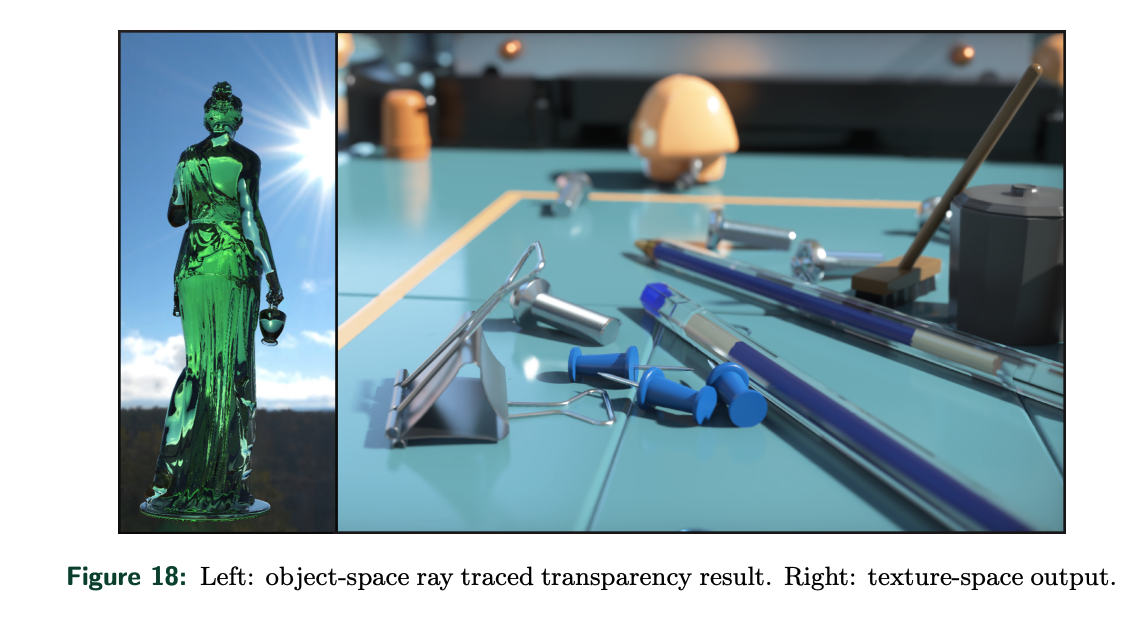
\includegraphics[height=0.7\textheight]{object-and-texture-space-transparency}
    \end{center}
    \begin{center}
        \small{Comparação: Transparência ray traced em espaço de objeto (esquerda) e resultado em espaço de textura (direita)}
    \end{center}
\end{frame}

\begin{frame}{Transparência com Ray Tracing}
    \begin{center}
        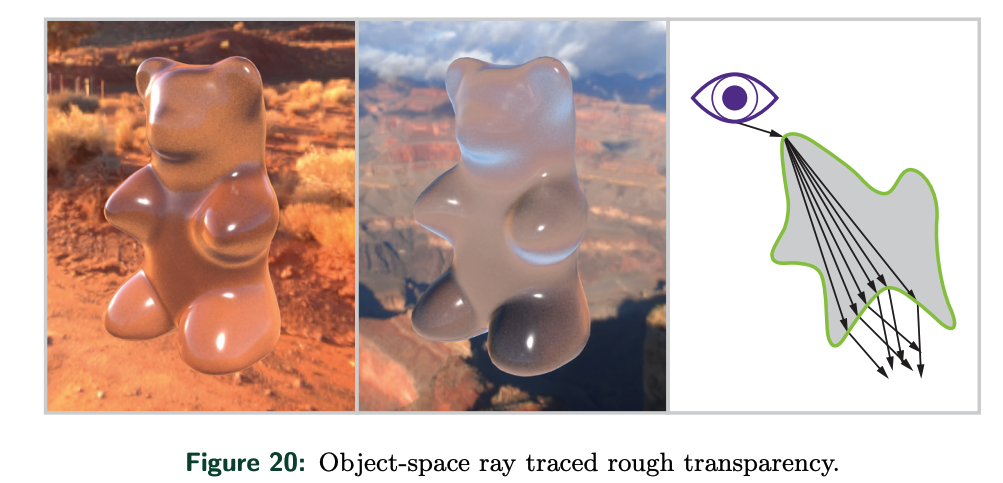
\includegraphics[height=0.7\textheight]{object-space-ray-traced-transparency}
    \end{center}
    \begin{center}
        \small{Transparência áspera com ray tracing: objeto original, transparência e diagrama de raios}
    \end{center}
\end{frame}

\begin{frame}{Efeitos de Translucidez}
    \begin{center}
        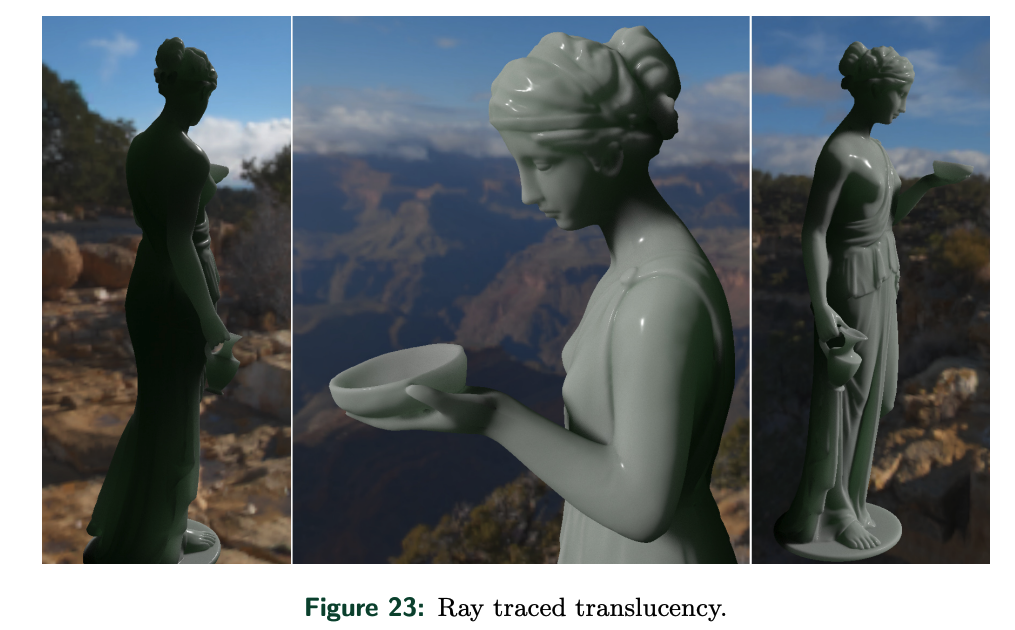
\includegraphics[width=0.95\textwidth]{ray-traced-translucency}
    \end{center}
    \begin{center}
        \small{Demonstração de translucidez com ray tracing em diferentes ângulos de visualização}
    \end{center}
\end{frame}

%=================================================
\section{Pipeline de Renderização}
%=================================================
\begin{frame}{Iluminação Global: Surfels para Resultados Dinâmicos}
    \begin{itemize}
        \item Surfels calculam iluminação indireta difusa sem pré-computação.
        \item Surfels são alocados dinamicamente, baseados em cobertura e área dos pixels.
        \item A irradiância é calculada por path tracing e acumulação temporal.
    \end{itemize}
    \begin{equation*}
        x_{n+1} = \text{lerp}(x_n, x_{n+1}, k)
    \end{equation*}
\end{frame}

\begin{frame}{Interreflexão Difusa Baseada em Surfels}
    \begin{center}
        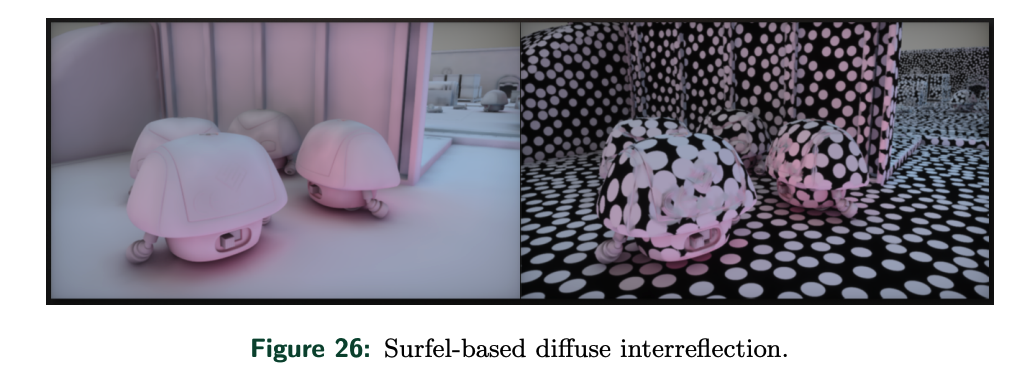
\includegraphics[height=0.7\textheight]{surfel-based-diffuse-interreflection}
    \end{center}
    \begin{center}
        \small{Demonstração de interreflexão difusa usando surfels: iluminação direta (esquerda) vs. iluminação global com surfels (direita)}
    \end{center}
\end{frame}

\begin{frame}{Comparação de Técnicas de Iluminação Global}
    \begin{center}
        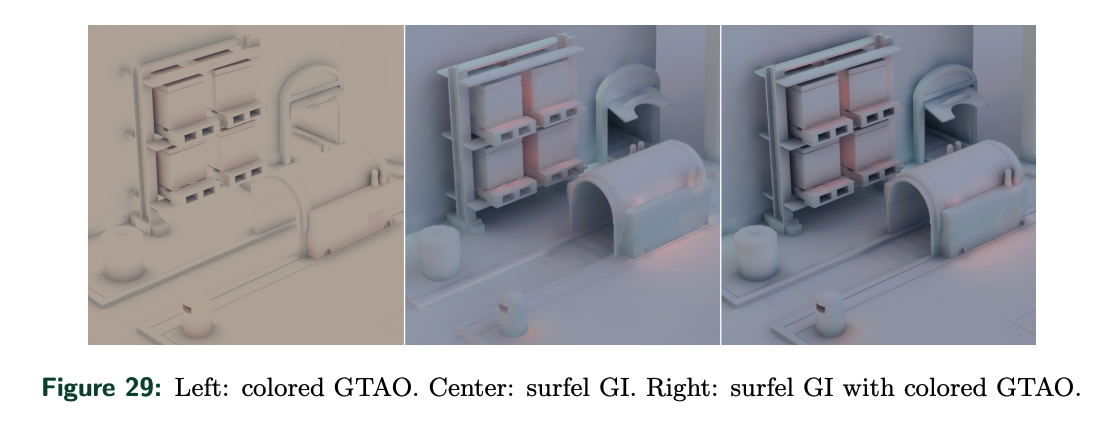
\includegraphics[width=0.95\textwidth]{surfel-comparacao}
    \end{center}
    \begin{center}
        \small{Comparação: GTAO colorido (esquerda), iluminação global com surfels (centro),\\
        e combinação de surfels com GTAO colorido (direita)}
    \end{center}
\end{frame}

\begin{frame}{Profundidade de Campo: Combinando Ray Tracing e Pós-Processamento}
    \begin{itemize}
        \item O ray tracing resolve o problema de semi-transparência em objetos fora de foco.
        \item Uma máscara de raios adaptativa concentra o ray tracing onde há maior necessidade.
        \item A variância temporal da luminância influencia a máscara de raios.
    \end{itemize}
    \begin{equation*}
        x_f = \text{saturate}(x_n + \sigma^2 \cdot 100000) \cdot m
    \end{equation*}
\end{frame}

\begin{frame}{Demarcação de Campo Próximo e Distante}
    \begin{center}
        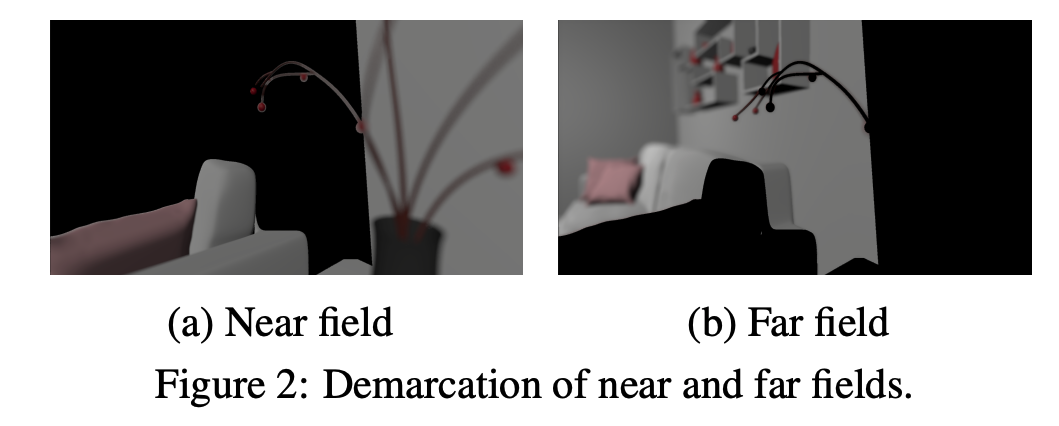
\includegraphics[width=0.95\textwidth]{near-far-field}
    \end{center}
    \begin{center}
        \small{Demonstração de (a) campo próximo e (b) campo distante na profundidade de campo}
    \end{center}
\end{frame}

\begin{frame}{Semi-transparências em Objetos Fora de Foco}
    \begin{center}
        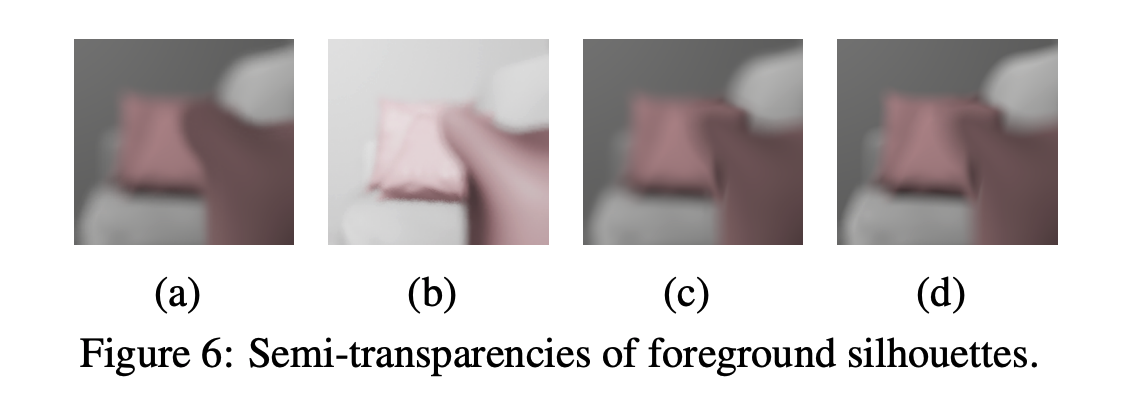
\includegraphics[width=0.95\textwidth]{semi-transparencias}
    \end{center}
    \begin{center}
        \small{Comparação de técnicas para semi-transparências em silhuetas de objetos em primeiro plano:\\
        (a) referência, (b) ray tracing, (c) pós-processamento, (d) híbrido}
    \end{center}
\end{frame}

\begin{frame}{Máscara de Raios Adaptativa}
    \begin{center}
        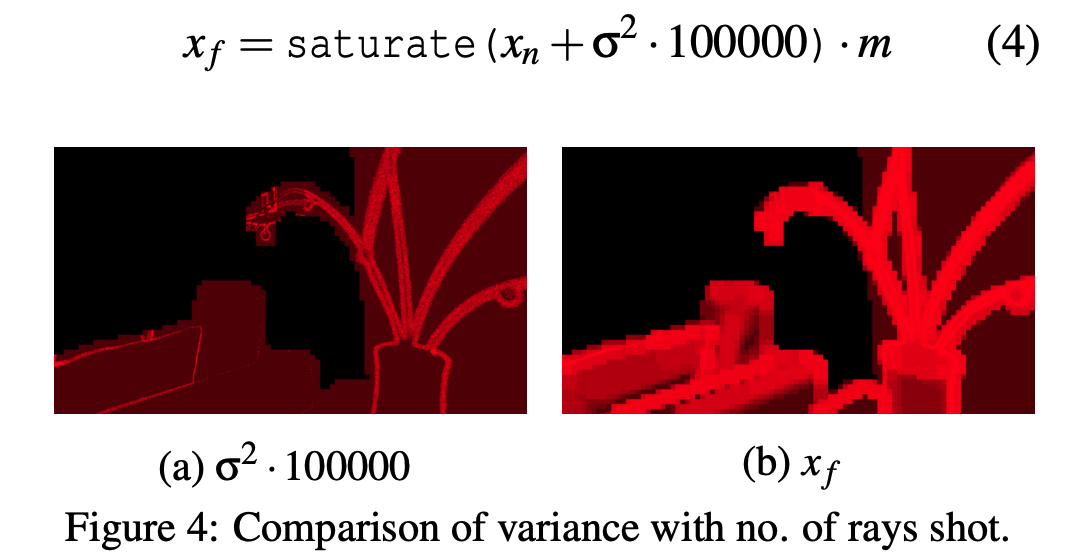
\includegraphics[width=0.95\textwidth]{mascara-raios-adaptativos}
    \end{center}
    \begin{center}
        \small{Comparação entre (a) variância ($\sigma^2 \cdot 100000$) e (b) máscara de raios final ($x_f$)}
    \end{center}
\end{frame}

\begin{frame}{Renderização Híbrida para Cenas Dinâmicas}
    \begin{itemize}
        \item Separamos a cena em componentes estáticos e dinâmicos.
        \item O transporte de luz é: cena estática + diferença causada por objetos dinâmicos.
        \item A diferença do transporte de luz é esparsa, possibilitando amostragem adaptativa.
    \end{itemize}
    \begin{equation*}
        L = L_s + (L_+ - L_-) \cdot s_i = s_t \cdot \frac{\text{Var}(L_{\Delta,i}) + |L_{\Delta,i}|}{\sum(\text{Var}(L_{\Delta,j}) + |L_{\Delta,j}|)}
    \end{equation*}
\end{frame}

\begin{frame}{Interação da Luz com Objetos Dinâmicos}
    \begin{center}
        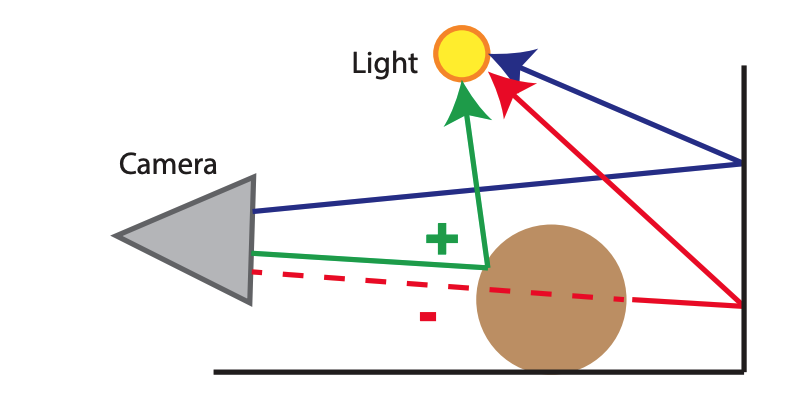
\includegraphics[height=0.7\textheight]{interacao-com-luz-objetos-dinamicos}
    \end{center}
    \begin{center}
        \small{Diagrama mostrando a interação da luz com objetos dinâmicos na cena}
    \end{center}
\end{frame}

\begin{frame}{Inserção de Objetos Dinâmicos}
    \begin{center}
        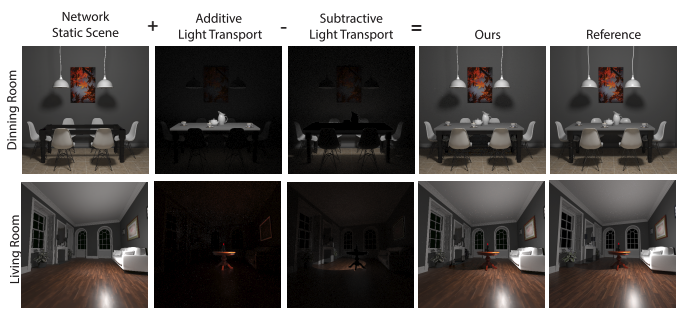
\includegraphics[width=0.95\textwidth]{insercao-objetos-dinamicos}
    \end{center}
    \begin{center}
        \small{Processo de inserção de objetos dinâmicos: cena estática + transporte de luz aditivo - transporte de luz subtrativo = resultado final}
    \end{center}
\end{frame}

\begin{frame}{Comparação com Path Tracing}
    \begin{center}
        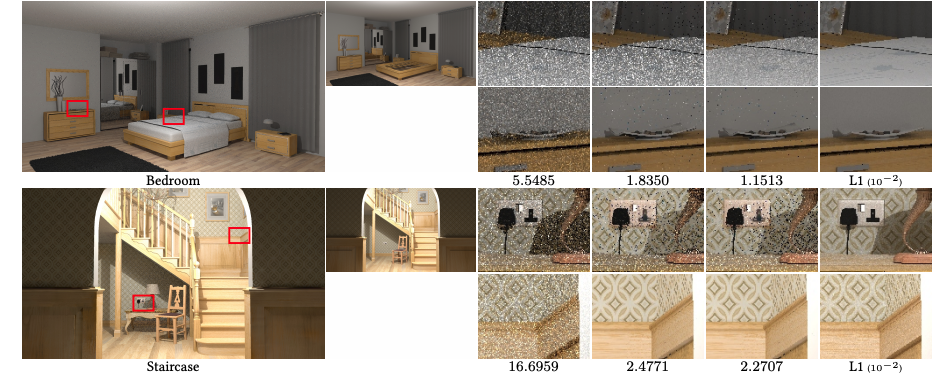
\includegraphics[width=0.95\textwidth]{comparacao-path-tracing}
    \end{center}
    \begin{center}
        \small{Comparação de convergência e qualidade visual entre diferentes técnicas de renderização}
    \end{center}
\end{frame}

%=================================================
\section{Técnicas de Renderização}
%=================================================
\subsection{Sombras e Reflexos}
\subsection{Oclusão Ambiente}
\subsection{Transparência e Translucidez}

%=================================================
\section{Iluminação Global}
%=================================================
\begin{frame}{Iluminação Global: Surfels para Resultados Dinâmicos}
    \begin{itemize}
        \item Surfels calculam iluminação indireta difusa sem pré-computação.
        \item Surfels são alocados dinamicamente, baseados em cobertura e área dos pixels.
        \item A irradiância é calculada por path tracing e acumulação temporal.
    \end{itemize}
    \begin{equation*}
        x_{n+1} = \text{lerp}(x_n, x_{n+1}, k)
    \end{equation*}
\end{frame}

\begin{frame}{Interreflexão Difusa Baseada em Surfels}
    \begin{center}
        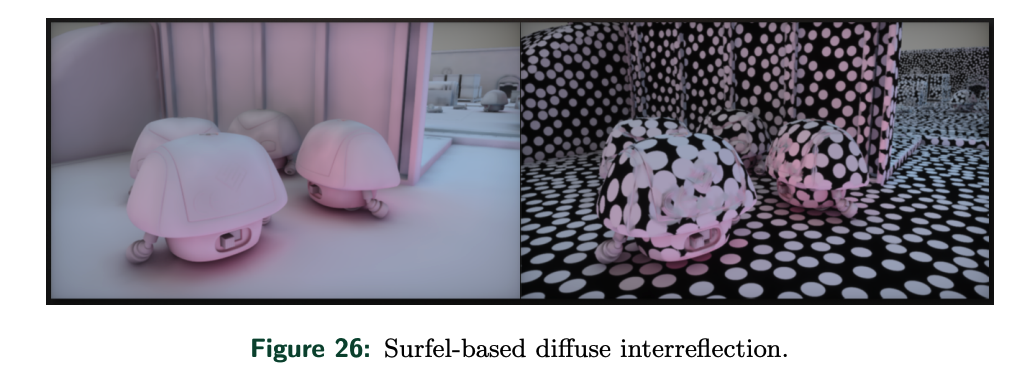
\includegraphics[height=0.7\textheight]{surfel-based-diffuse-interreflection}
    \end{center}
    \begin{center}
        \small{Demonstração de interreflexão difusa usando surfels: iluminação direta (esquerda) vs. iluminação global com surfels (direita)}
    \end{center}
\end{frame}

\begin{frame}{Comparação de Técnicas de Iluminação Global}
    \begin{center}
        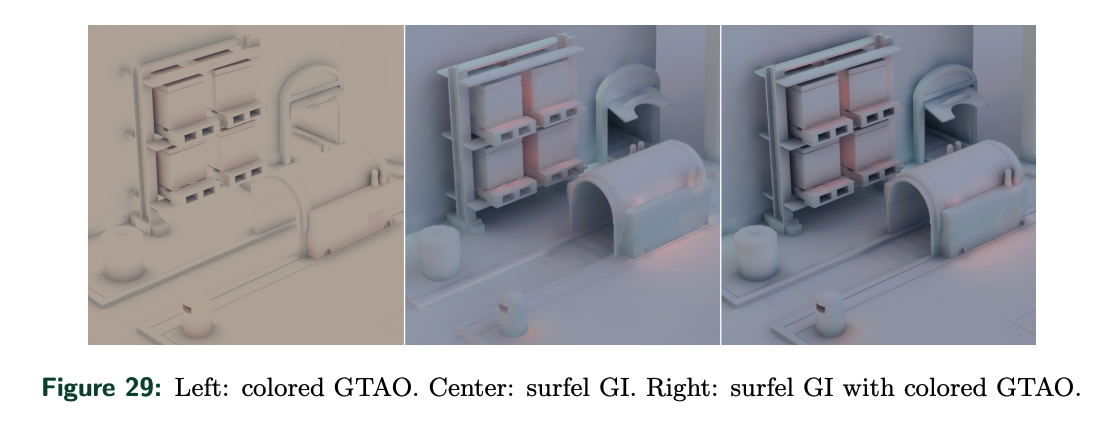
\includegraphics[width=0.95\textwidth]{surfel-comparacao}
    \end{center}
    \begin{center}
        \small{Comparação: GTAO colorido (esquerda), iluminação global com surfels (centro),\\
        e combinação de surfels com GTAO colorido (direita)}
    \end{center}
\end{frame}

%=================================================
\section{Otimizações e Desempenho}
%=================================================
\subsection{Profundidade de Campo}
\subsection{Cenas Dinâmicas}
\subsection{Métricas de Desempenho}

\begin{frame}{Desempenho e Qualidade Visual}
    \begin{itemize}
        \item A renderização híbrida aumenta o desempenho com melhor qualidade visual.
        \item A qualidade visual se aproxima do ray tracing, com menor custo computacional.
        \item Atinge qualidade de path tracing offline em tempo real com alocação inteligente de raios.
        \item \textbf{Destaque:} A renderização híbrida pode ter um desempenho até 6x superior ao path tracing tradicional.
    \end{itemize}
    % Espaço para tabelas de desempenho
    \begin{center}
        \framebox[0.8\textwidth]{\parbox{0.7\textwidth}{\centering [Tabelas: Métricas de Desempenho]}}
    \end{center}
\end{frame}

%=================================================
\section{Conclusão}
%=================================================
\begin{frame}{Conclusão: O Futuro da Renderização Híbrida}
    \begin{itemize}
        \item A renderização híbrida oferece qualidade visual aprimorada e desempenho otimizado.
        \item Há grande potencial para futuras aplicações e melhorias.
        \item A renderização híbrida é o futuro da renderização em tempo real.
    \end{itemize}
    % Espaço para imagem futurística
    \begin{center}
        \framebox[0.8\textwidth]{\parbox{0.7\textwidth}{\centering [Imagem: Visão Futurística]}}
    \end{center}
\end{frame}

%=================================================
\section{Referências}
%=================================================
\begin{frame}[allowframebreaks]{Referências}
    \nocite{*}
    \printbibliography[heading=none]
\end{frame}

\end{document}